\documentclass{article}

% -----------------------------
% Packages
% -----------------------------
\usepackage{fancyhdr}
\usepackage{extramarks}
\usepackage{amsmath}
\usepackage{amsthm}
\usepackage{amsfonts}
\usepackage{tikz}
\usepackage[plain]{algorithm}
\usepackage{algpseudocode}
\usepackage{amssymb}
\usepackage{graphicx}

\usetikzlibrary{automata,positioning}

% -----------------------------
% Basic Document Settings
% -----------------------------
\topmargin=-0.45in
\evensidemargin=0in
\oddsidemargin=0in
\textwidth=6.5in
\textheight=9.0in
\headsep=0.25in

\linespread{1.1}

\pagestyle{fancy}
\lhead{\hmwkAuthorName}
\chead{\hmwkClass: \hmwkTitle}
\rhead{}
\lfoot{\lastxmark}
\cfoot{\thepage}

\renewcommand\headrulewidth{0.4pt}
\renewcommand\footrulewidth{0.4pt}

\setlength\parindent{0pt}

% -----------------------------
% Problem Section Helpers
% -----------------------------
\newcommand{\enterProblemHeader}[1]{
  \nobreak\extramarks{}{Problem \arabic{#1} continued on next page\ldots}\nobreak{}
  \nobreak\extramarks{Problem \arabic{#1} (continued)}{Problem \arabic{#1} continued on next page\ldots}\nobreak{}
}

\newcommand{\exitProblemHeader}[1]{
  \nobreak\extramarks{Problem \arabic{#1} (continued)}{Problem \arabic{#1} continued on next page\ldots}\nobreak{}
  \stepcounter{#1}
  \nobreak\extramarks{Problem \arabic{#1}}{}\nobreak{}
}

\setcounter{secnumdepth}{0}
\newcounter{partCounter}
\newcounter{homeworkProblemCounter}
\setcounter{homeworkProblemCounter}{1}
\nobreak\extramarks{Problem \arabic{homeworkProblemCounter}}{}\nobreak{}

% -----------------------------
% Theorem env (optional)
% -----------------------------
\newtheorem*{theorem}{Theorem}

% -----------------------------
% Homework Problem Environment
%   Usage:
%   \begin{homeworkProblem}            % auto-number
%     % Your answer here
%   \end{homeworkProblem}
%
%   \begin{homeworkProblem}[7]         % set problem number to 7
%     % Your answer here
%   \end{homeworkProblem}
% -----------------------------
\newenvironment{homeworkProblem}[1][-1]{
  \ifnum#1>0
    \setcounter{homeworkProblemCounter}{#1}
  \fi
  \section{Problem \arabic{homeworkProblemCounter}}
  \setcounter{partCounter}{1}
  \enterProblemHeader{homeworkProblemCounter}
}{
  \exitProblemHeader{homeworkProblemCounter}
}

% -----------------------------
% Homework Details (EDIT THESE)
% -----------------------------
\newcommand{\hmwkTitle}{Homework \ 3}
\newcommand{\hmwkClass}{CS 4262}
\newcommand{\hmwkClassInstructor}{Prof. Dr. Thomas Beckers}
\newcommand{\hmwkAuthorName}{\textbf{Joseph Quinn}}

% -----------------------------
% Title
% -----------------------------
\title{
  \vspace{2in}
  \textmd{\textbf{\hmwkClass:\ \hmwkTitle}}\\
  \vspace{0.1in}\large{\textit{\hmwkClassInstructor\ }}
  \vspace{3in}
}
\author{\hmwkAuthorName}
\date{}

% -----------------------------
% Convenience Macros (optional)
% -----------------------------
\renewcommand{\part}[1]{\textbf{\large Part \Alph{partCounter}}\stepcounter{partCounter}\\}

% Algorithms
\newcommand{\alg}[1]{\textsc{\bfseries \footnotesize #1}}

% Calculus
\newcommand{\deriv}[1]{\frac{\mathrm{d}}{\mathrm{d}x} (#1)}
\newcommand{\pderiv}[2]{\frac{\partial}{\partial #1} (#2)}
\newcommand{\dx}{\mathrm{d}x}

% Statistics
\newcommand{\E}{\mathrm{E}}
\newcommand{\Var}{\mathrm{Var}}
\newcommand{\Cov}{\mathrm{Cov}}
\newcommand{\Bias}{\mathrm{Bias}}

% Proof step (for aligned derivations)
\newcommand{\step}[2]{& #1 & & \text{#2} \\}

% Solution header (optional)
\newcommand{\solution}{\textbf{\large Solution}}

% -----------------------------
% Document
% -----------------------------
\begin{document}

\maketitle
\pagebreak

\begin{homeworkProblem}
	\subsection{1.1}
	$d(u,v) =\|u - v\|^2$
	We then expand this into \[
		u^Tu - 2vu + v^Tv
	\]
	Using a kernel function $K(x,z) = \phi{(x), \phi{(z)}}$. We can rewrite this as:
	\[
		K(u,u) -2K(u,v) + K(v,v)
	\]

	We know the euclidian distance expands to:
	\[
		d_{\text{euc}}(x^{(i)}, x^{(j)}) = \|x^{(i)} - x^{(j)}\|^2
		= x^{(i)T}x^{(i)} + x^{(j)T}x^{(j)} - 2\,x^{(i)T}x^{(j)}
	\]

	So for a linear kernel: $K(x,z) = x^\top z$

	We get the same result as the euclidian distance formula:

	\[
		d_{k}(x^{(i)}, x^{(j)}) = x^{(i)T}x^{(i)} + x^{(j)T}x^{(j)} - 2\,x^{(i)T}x^{(j)}
	\]



	\subsection{1.2}

	\begin{figure}[h]
		\centering
		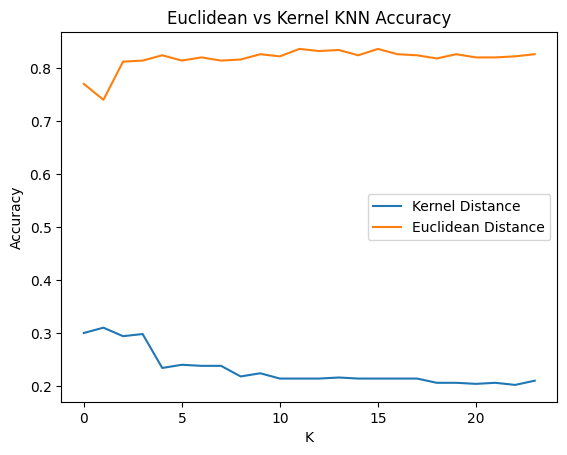
\includegraphics[width=0.4\textwidth]{../../imgs/hw3_1.2.png}
	\end{figure}

\end{homeworkProblem}

\pagebreak

\begin{homeworkProblem}
	\subsection*{2.1}
	
	\begin{figure}[h]
		\centering

		% Polynomial (p1-p5)
		\begin{tabular}{ccccc}
			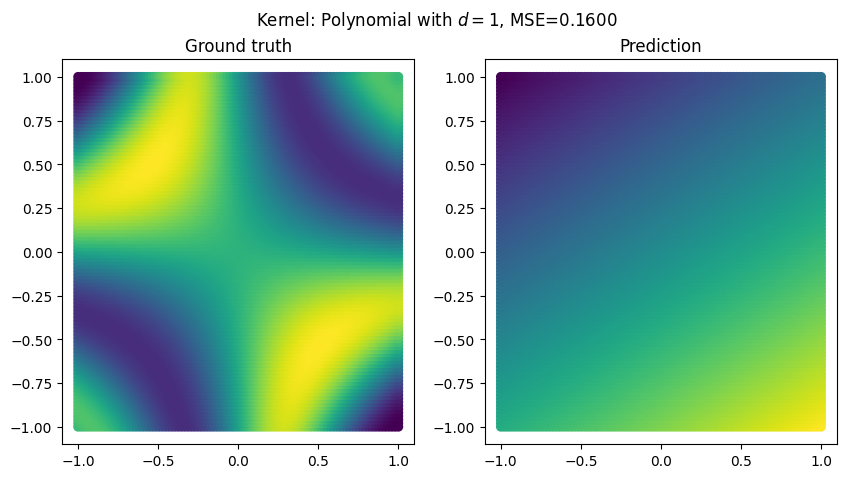
\includegraphics[width=0.18\textwidth]{../../imgs/hw3_2.1_p1.png} &
			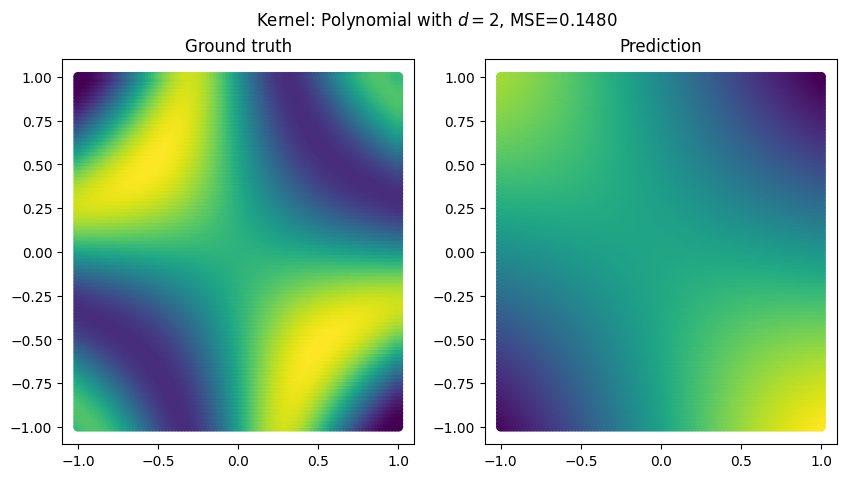
\includegraphics[width=0.18\textwidth]{../../imgs/hw3_2.1_p2.png} &
			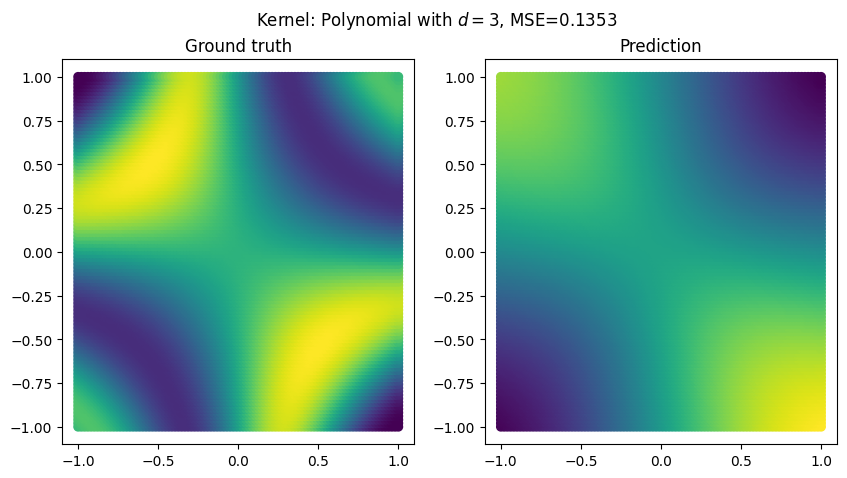
\includegraphics[width=0.18\textwidth]{../../imgs/hw3_2.1_p3.png} &
			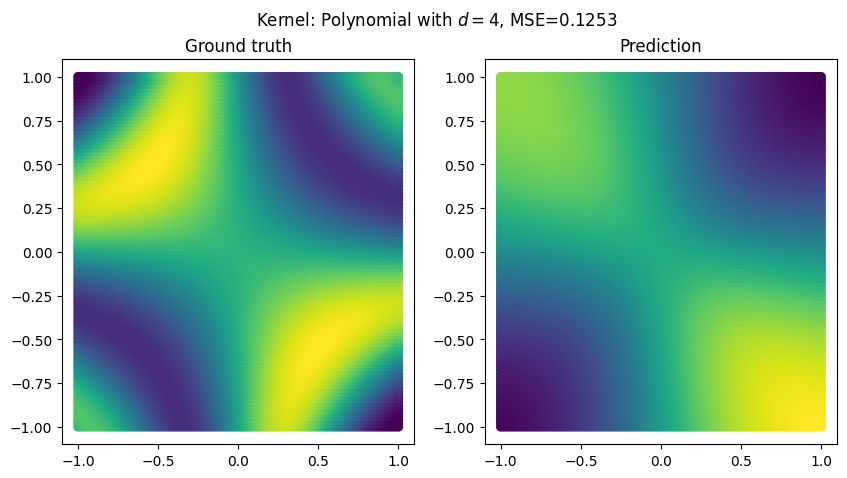
\includegraphics[width=0.18\textwidth]{../../imgs/hw3_2.1_p4.png} &
			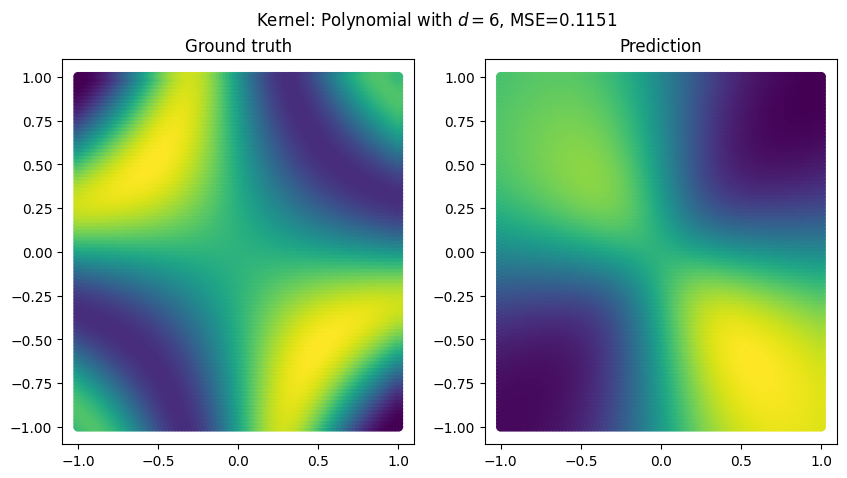
\includegraphics[width=0.18\textwidth]{../../imgs/hw3_2.1_p5.png}   \\
		\end{tabular}
		\vspace{4pt}
		\\
		\textit{Polynomial Kernel Results (d = 1, 2, 3, 4, 6)}

		\vspace{8pt}

		% RBF (p6-p9)
		\begin{tabular}{cccc}
			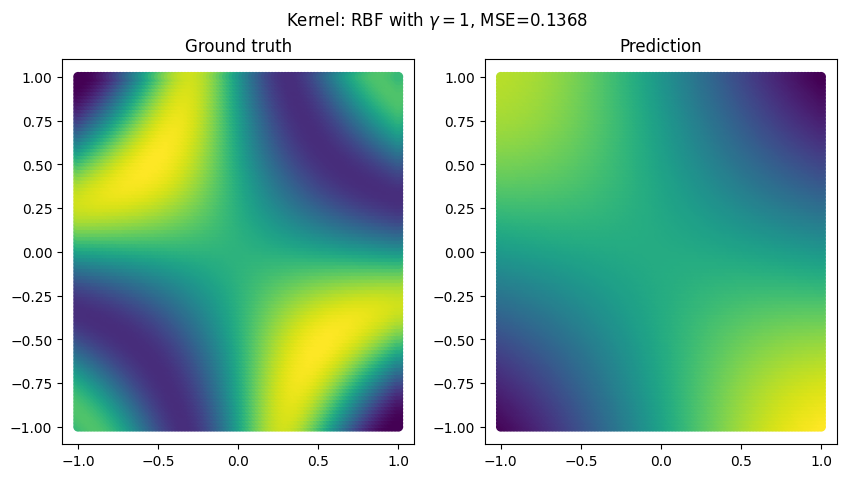
\includegraphics[width=0.22\textwidth]{../../imgs/hw3_2.1_p6.png} &
			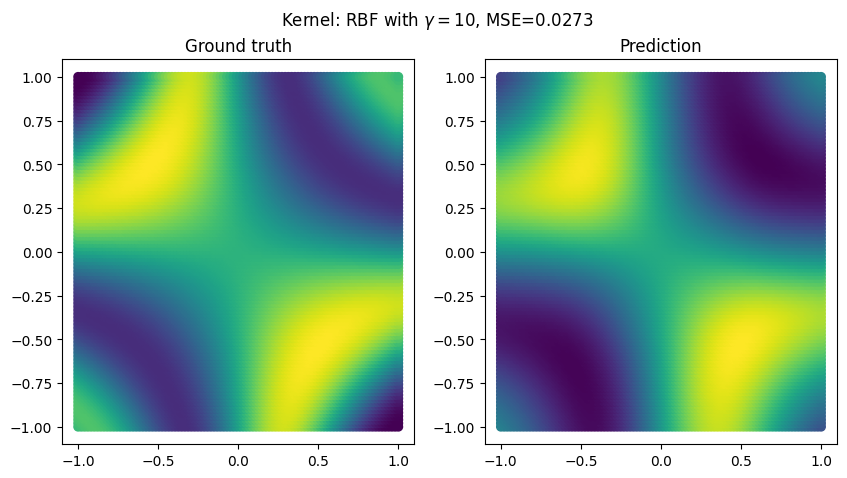
\includegraphics[width=0.22\textwidth]{../../imgs/hw3_2.1_p7.png} &
			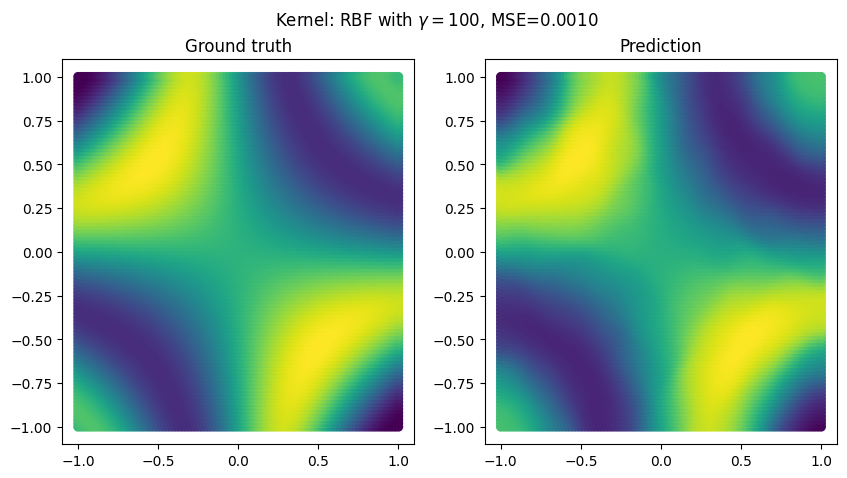
\includegraphics[width=0.22\textwidth]{../../imgs/hw3_2.1_p8.png} &
			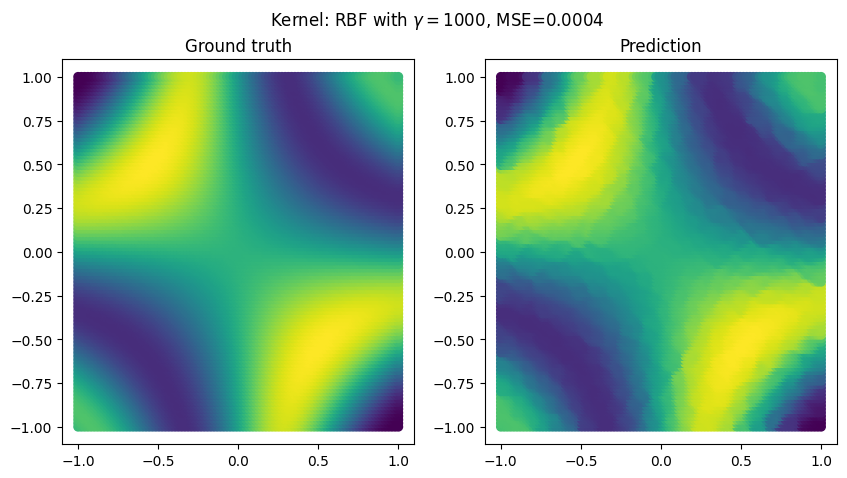
\includegraphics[width=0.22\textwidth]{../../imgs/hw3_2.1_p9.png}   \\
		\end{tabular}
		\vspace{4pt}
		\\
		\textit{RBF Kernel Results ($\gamma$ = 1, 10, 100, 1000)}

		\vspace{8pt}

		% Custom (p10-p13)
		\begin{tabular}{cccc}
			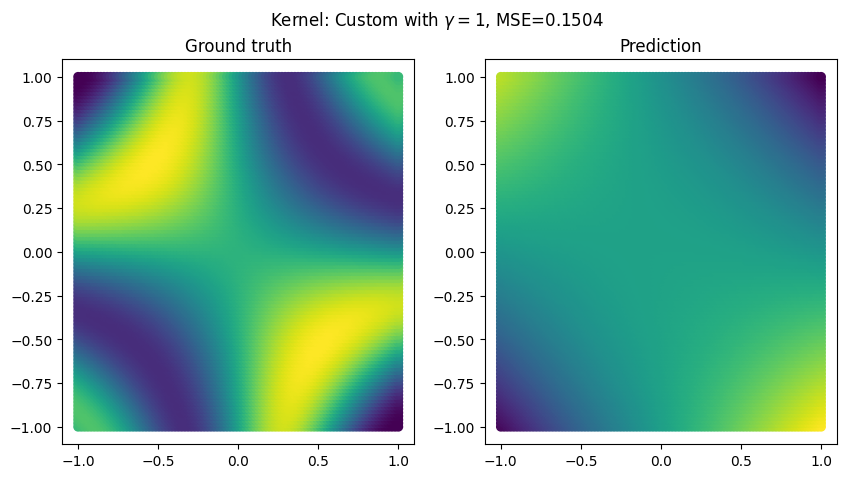
\includegraphics[width=0.22\textwidth]{../../imgs/hw3_2.1_p10.png} &
			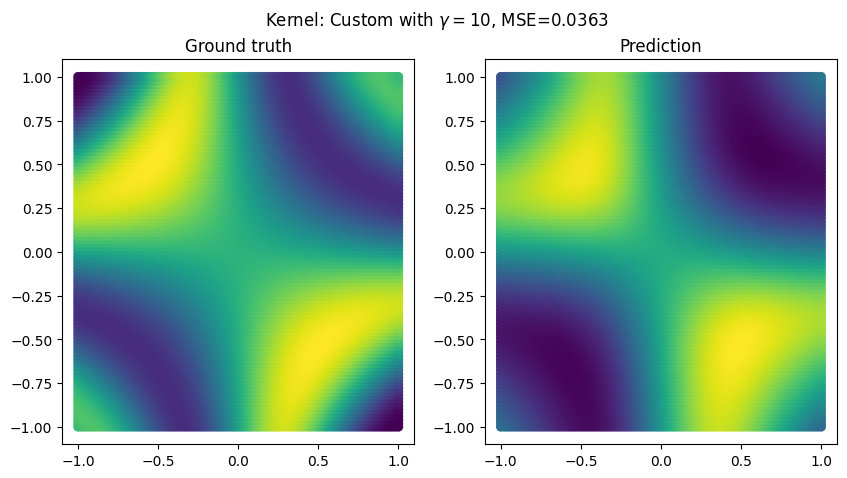
\includegraphics[width=0.22\textwidth]{../../imgs/hw3_2.1_p11.png} &
			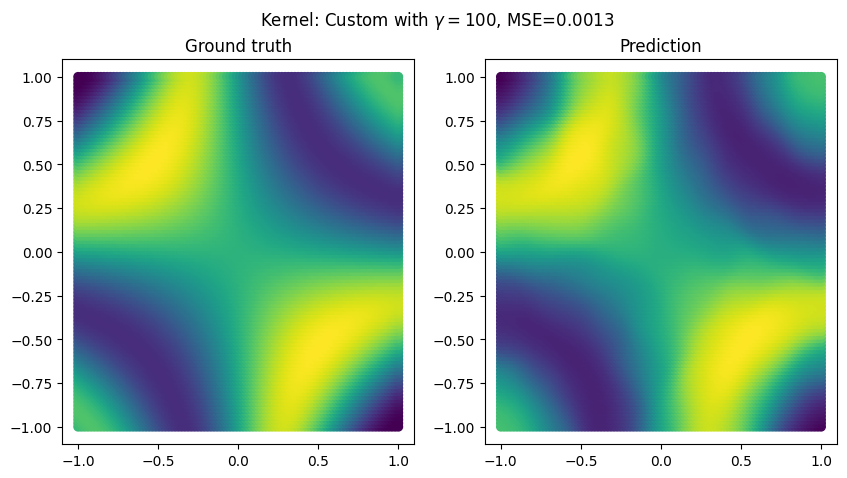
\includegraphics[width=0.22\textwidth]{../../imgs/hw3_2.1_p12.png} &
			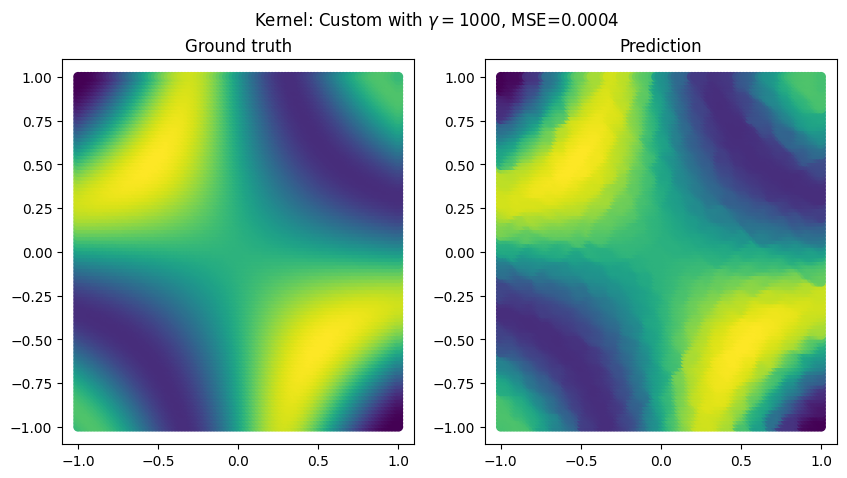
\includegraphics[width=0.22\textwidth]{../../imgs/hw3_2.1_p13.png}   \\
		\end{tabular}
		\vspace{4pt}
		\\
		\textit{Custom Kernel Results ($\gamma$ = 1, 10, 100, 1000)}

		\caption{Non-parametric regression outputs for Polynomial, RBF, and Custom kernels}
	\end{figure}

	\subsection*{2.2}
	\textbf{Original KNN Average Time: } 72.25 seconds \\
	\textbf{LSH KNN Average Time: } 9.15 seconds

\end{homeworkProblem}

\pagebreak

\begin{homeworkProblem}
	\subsection*{3.1}
	i) Maximizing projection variance:
	\[
		\mathrm{var} = \frac{1}{N} \sum_{i=1}^{N} (z_i - \bar{z})^2
		= \frac{1}{N} \sum_{i=1}^{N} \left( \mathbf{w}^T (\mathbf{x}_i - \bar{\mathbf{x}}) \right)^2
	\]

	\[
		\text{var} = \frac{1}{N} \sum_{i=1}^{N} \left(w^T(x_i - \bar{x})\right)^2
		= \frac{1}{N} \sum_{i=1}^{N} w^T(x_i - \bar{x})(x_i - \bar{x})^T w
	\]

	\[
		= w^T \left( \frac{1}{N} \sum_{i=1}^{N} (x_i - \bar{x})(x_i - \bar{x})^T \right) w
		= w^T S w
	\]

	\[
		\text{Therefore maximizing the variance can be written as:}
	\]

	\[
		\max_{w} \quad w^T S w
	\]


	ii) Minimizing reconstruction error:

	In order to reconstruct from $z \rightarrow x$ we see the following:

	\[
		\hat{x} = w w^T x
	\]

	Now we can write the reconstruction error as:

	\begin{align}
		\frac{1}{N} \sum_{i=1}^{N} \left\| \hat{x}^{(i)} - x^{(i)} \right\|^2
		 & = \frac{1}{N} \sum_{i=1}^{N} \left\| ww^T x^{(i)} - x^{(i)} \right\|^2
	\end{align}

	We can further simplify:
	\[
		\begin{aligned}
			\min_{w} \;   & \frac{1}{N} \sum_{i=1}^{N} \left\| ww^T x^{(i)} - x^{(i)} \right\|^2 \\
			= \min_{w} \; & \frac{1}{N} \sum_{i=1}^{N} (ww^T x_i - x_i)^T (ww^T x_i - x_i)       \\
			= \min_{w} \; & \frac{1}{N} \sum_{i=1}^{N} x_i^T ww^T ww^T x_i - 2x_i^T ww^T x_i     \\
			= \min_{w} \; & -\frac{1}{N} \sum_{i=1}^{N} x_i^T ww^T x_i                           \\
			= \min_{w} \; & - w^T \left( \frac{1}{N} \sum_{i=1}^{N} x_i x_i^T \right) w          \\
			= \max_{w} \; & w^T S w
		\end{aligned}
	\]

	\emph{Both approaches lead to the same optimization problem:}
	\[
		\max_{w} \quad w^T S w \quad \text{subject to} \quad w^T w = 1
	\]
	\emph{The optimal solution $w^*$ is the eigenvector of $S$ corresponding to the largest eigenvalue.}

	\subsection*{3.2}
	
\begin{figure}[H]
		\centering
		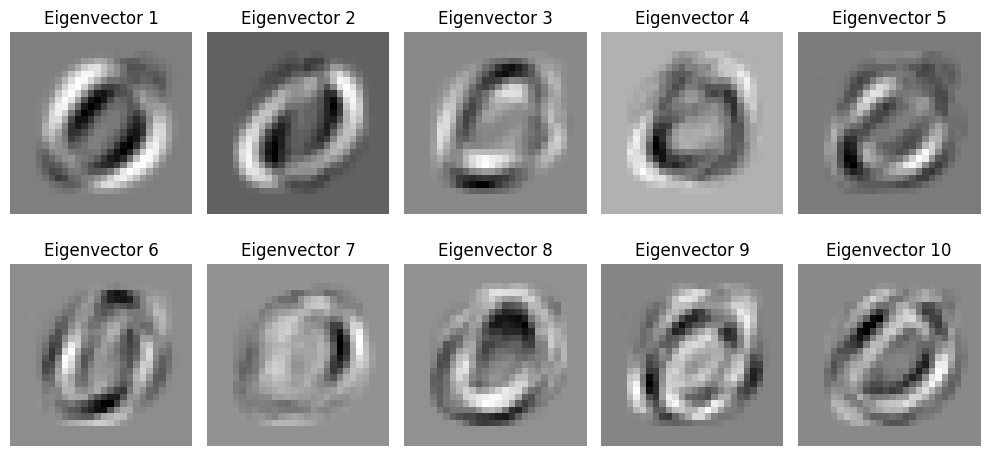
\includegraphics[width=0.7\textwidth]{../../imgs/hw3_3.2.png}
	\end{figure}

\subsection*{3.3}

	\begin{figure}[H]
		\centering
		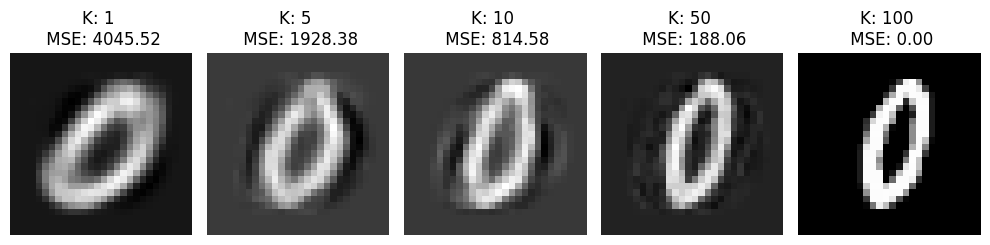
\includegraphics[width=0.7\textwidth]{../../imgs/hw3_3.3.png}
	\end{figure}


\end{homeworkProblem}

\end{document}
